El sistema permite el ajuste de una serie de parámetros para permitir al usuario jugar con estos y ver sus efectos en el modelo entrenado:

\textbf{Parámetros de la formación de transformadas de Fourier}
\begin{itemize}
    \item Tamaño de la ventana STFT.
    \item Desplazamiento entre ventanas STFT.
    \item Tipo de ventana utilizada para la STFT.
\end{itemize}

\textbf{Parámetros intrínsecos del modelo}
\begin{itemize}
    \item Número de canales de entrada (Mono / Estéreo).
    \item Porcentaje de \textit{dropout}.
    \item Función de activación para la capa de salida.
\end{itemize}

\textbf{Parámetros de efectos para entrenamiento y de audio}
\begin{itemize}
    \item Prob. de aplicar efectos (reverb,pitch,shift,noise ... ).
    \item Nivel de ruido.
    \item Frecuencia de muestreo (sample rate).
    \item Ref. en decibelios para normalizar espectrogramas
    \item Normalización de audio (recomendable si los datos vienen de diferentes fuentes).
\end{itemize}

\textbf{Parámetros de entrenamiento}
\begin{itemize}
    \item \textit{Learning Rate}.
    \item \textit{Batch Size}.
    \item Épocas.
    \item Tamaño de las épocas.
    \item \textit{Gradient clip}.
    \item \textit{Weight decay}
\end{itemize}

\textbf{Parámetros de generación de mezclas}
\begin{itemize}
    \item \textit{Coherent prob}
\end{itemize}

Además, se introduce otra pestaña adicional, donde se da información sobre lo que es cada parámetro

\begin{figure}[H]
    \centering

    \begin{subfigure}{0.45\textwidth}
        \centering
        
\includegraphics[width=\textwidth,height=0.55\textheight,keepaspectratio]{commons/BotónAyudaParametros.png}
        \caption{Botón para acceder a la ventana de información sobre los parámetros}
        \label{fig:boton-ayuda-gui}
    \end{subfigure}
    \hfill
    \begin{subfigure}{0.45\textwidth}
        \centering
        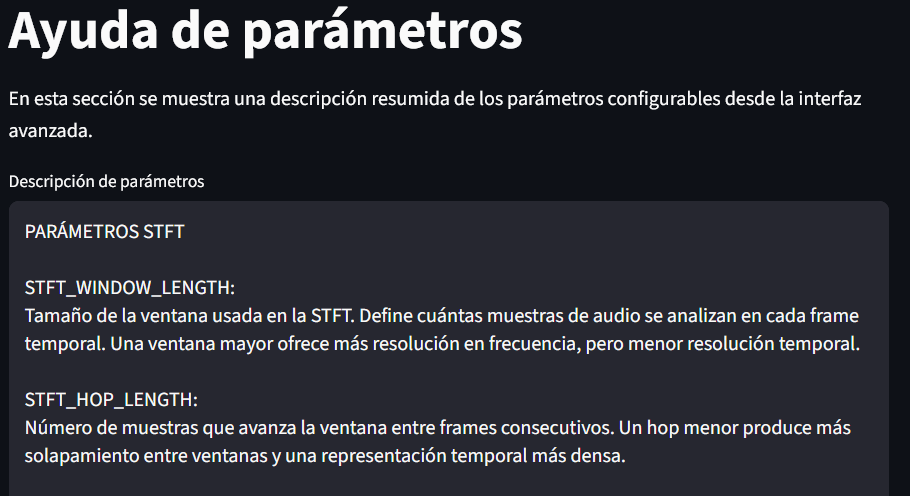
\includegraphics[width=\textwidth,height=0.55\textheight,keepaspectratio]{commons/AyudaParametros.png}
        \caption{Captura sobre la información de los parámetros}
        \label{fig:ayuda-params-gui}
    \end{subfigure}

    \caption{Entrada a la ventana de información sobre los parámetros de la configuración avanzada}
    \label{fig:informacion-parametros-gui}
\end{figure}



